\section{Introduction}

% Overview
  % Environmental mapping, what is the motivation?
  % Maps
  % RGBD sensors
% Goal

\subsection{Overview}

\begin{frame}{Overview} % ____________________________________________________
  \only<1>{
  Motivation for this work: provide a map of the environment \\ \medskip
  Examples applications:
  \begin{itemize}
    \item Autonomous agents (robots)
    \item Teleoperation (human)
  \end{itemize}
  }
  \only<2>{
  In the literature this is referred to as the SLAM problem
  \begin{itemize}
    \item Simultaneous Localization and Mapping
    \item Environmental Mapping
    \item Research began around 1987
    \item Sensing and computing technology
  \end{itemize}
  }
  \begin{center}
    \includegraphics[width=\textwidth]<3>{../figures/intro_goal.pdf}
  \end{center}

  \note<1>{\begin{itemize}
    \item Examples Autonomous
    \item - Path planning, obstacle avoidance, object manipulation
    \item Examples Teleoperation
    \item - Search and Rescue, Hazardous Environments
  \end{itemize}}
  \note<2>{\begin{itemize}
    \item Most work in this area describe the SLAM problem
    \item - Simultaneously locate the robot in the environment as well as map the
    environment
    \item Environmental Mapping
    \item - Deals specifically with the mapping part of the SLAM problem
    \item - This work is a contribution to Environmental Mapping
    \item 1987
    \item - Work in this area has been going on for more than 20 years
    \item Recent work
    \item - Rich and dense maps of the environment
    \item - Fueled by recent advances in sensing and computational power
  \end{itemize}}
  \note<3>{\begin{itemize}
    \item For this work
    \item Goal was to transform depth images into a mesh representation
    \item * I will explain these two components
    \item Depth images
    \item - each pixel represents distance from sensor instead of color
    \item Mesh representation
    \item - Vertices and elements
    \item - 3D points and the connects between those points
  \end{itemize}}
\end{frame}

\subsection{RBG-D Sensor}

\begin{frame}{RBG-D Sensor} % __________________________________________________
  \begin{center}
    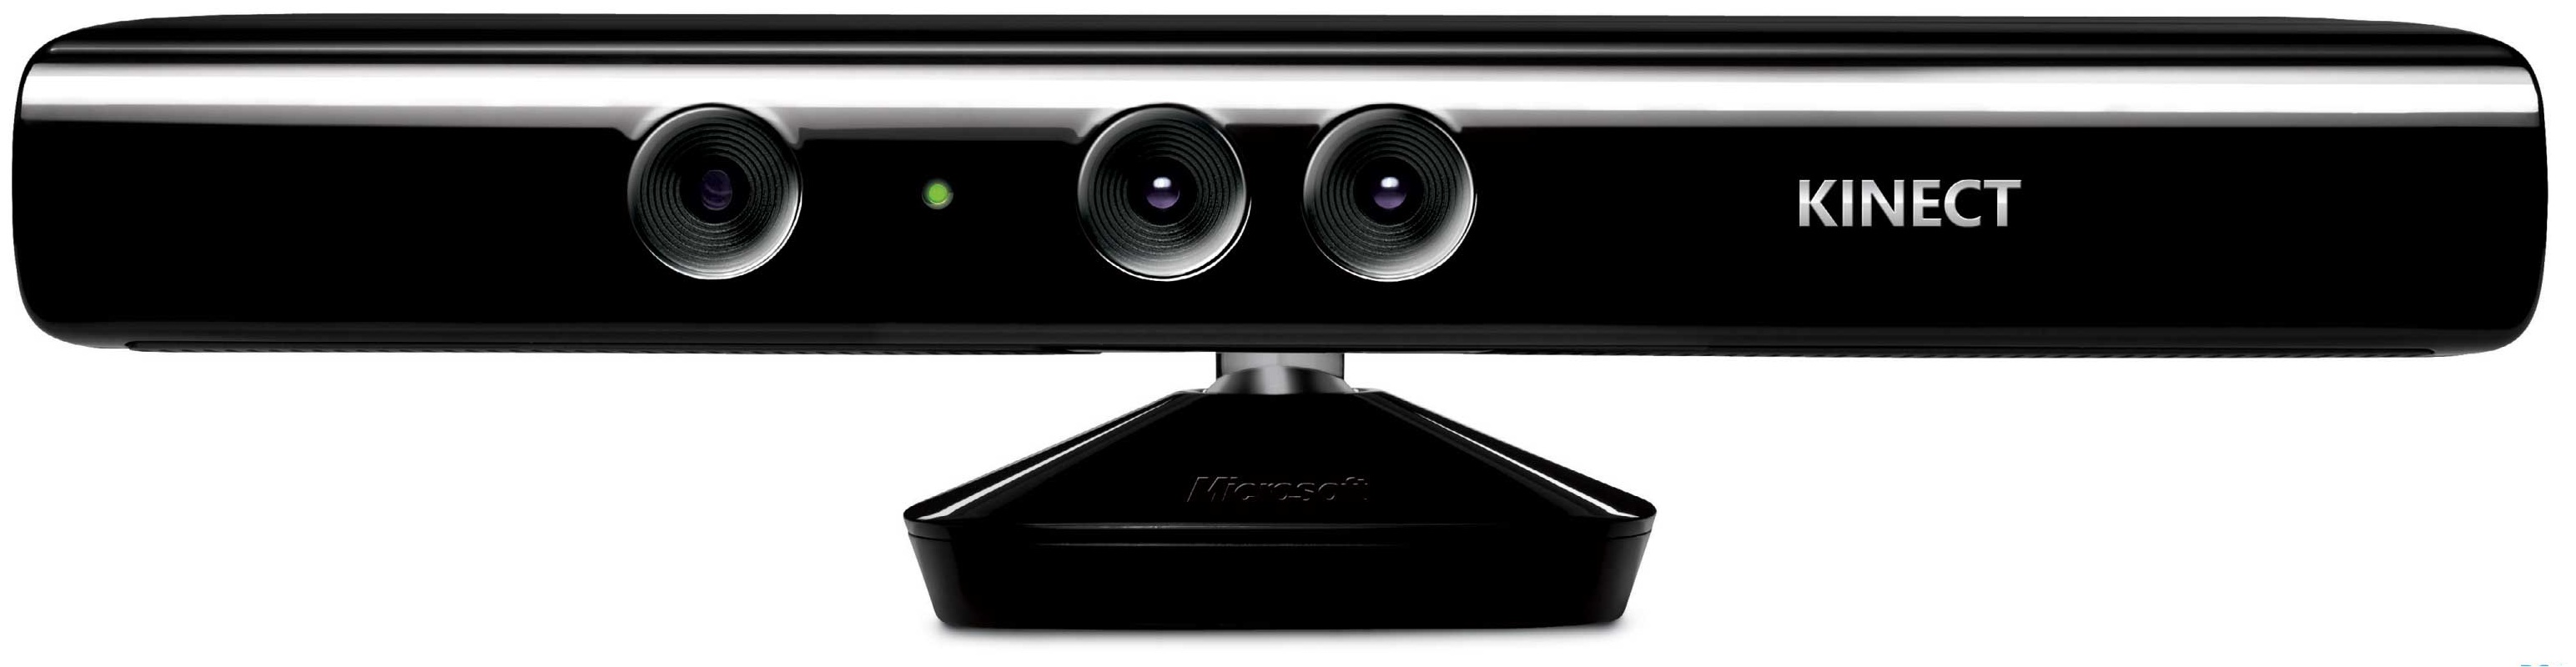
\includegraphics[width=\textwidth]{../figures/presentation/intro_kinect.jpeg}
  \end{center}
  \begin{itemize}
    \item 30 frames per second
    \item D - 9 million pixel values per second
    \item Algorithms must handle a high rate of data
  \end{itemize}

  \note{\begin{itemize}
    \item Kinect
    \item First affordable sensor to provide
    \item high resolution spatial information
    \item[]
    \item High rate of data
    \item Algorithms must have this as a design consideration
  \end{itemize}}
\end{frame}

\subsection{Map}

\begin{frame}{Mesh} % __________________________________________________
  \begin{center}
    \includegraphics[width=\textwidth]<1>{../figures/presentation/intro_mesh.png}
  \end{center}
  \only<2>{
  \begin{itemize}
    \item Supported
    \item Computationally Inexpensive
    \item Low Memory Requirement
  \end{itemize}
  }

  \note<1>{\begin{itemize}
    \item There are different types of maps
    \item Mesh is the map type chosen for this work
  \end{itemize}}
  \note<2>{\begin{itemize}
    \item Supported
    \item - available software, tools, research, algorithms, etc., for
    this type of map
    \item Computationally Inexpensive
    \item - GPUs make this computationally efficient
    \item Low Memory Requirement
    \item - Can it run on a laptop with a standard amount of RAM?
  \end{itemize}}
\end{frame}

\subsection{Contribution}

\begin{frame}{Pipeline} % ______________________________________________
  \hspace*{-12.5mm}
  \includegraphics[width=1.2\textwidth]<1>
    {../figures/intro_general_pipeline_blackbox.pdf}
  \includegraphics[width=1.2\textwidth]<2>
    {../figures/intro_general_pipeline_mabdi.pdf}

  \note<1>{\begin{itemize}
    \item Traditional Mesh-Based Mapping Methods
    \item - Take incoming data
    \item - Generate a mesh structure
    \item - Append to growing global mesh structure
  \end{itemize}}

  \note<2>{\begin{itemize}
    \item MABDI
    \item - Takes what we already know
    \item (the global mesh structure)
    \item - Uses it to throwaway points in the data that are redundant
    \item Ability to classify incoming data and only use what is novel
    \item is MABDI's contribution
  \end{itemize}}
\end{frame}

\begin{frame}{Contribution} % ______________________________________________
  MABDI's algorithmic design identifies redundant information and removes it
  \emph{before} it is added to the global mesh.
\end{frame}
